\documentclass[aspectratio=169]{beamer}

\usepackage{lmodern}
\usepackage[utf8]{inputenc}
\usepackage[T1]{fontenc}
\DeclareUnicodeCharacter{2A53}{$\land$}
\DeclareUnicodeCharacter{2A54}{$\lor$}
\DeclareUnicodeCharacter{27F9}{$\implies$}
\DeclareUnicodeCharacter{27FA}{$\iff$}
\DeclareUnicodeCharacter{22D3}{$\cup$}
\graphicspath{{assets/}}

\usetheme{metropolis} 
\setbeamertemplate{navigation symbols}{}
\titlegraphic{\includegraphics[height=1cm]{lambda.png}}

\title{Stating the Obvious}
\date{September 2022}
\author{boxy}

\usepackage{epigraph}
\setlength\epigraphwidth{.8\textwidth}
\setlength\epigraphrule{0pt}

\usepackage{syntax}
\usepackage{cprotect}
\usepackage{minted} 
\usepackage{ebproof}

\usepackage{tikz}
\usepackage{tikz-qtree}
\usetikzlibrary{automata, arrows.meta, positioning, decorations, decorations.pathreplacing}
\usetikzlibrary{positioning, calc}


\usepackage{etoolbox,xpatch}
\makeatletter
\AtBeginEnvironment{minted}{\dontdofcolorbox}
\def\dontdofcolorbox{\renewcommand\fcolorbox[4][]{##4}}
\xpatchcmd{\inputminted}{\minted@fvset}{\minted@fvset\dontdofcolorbox}{}{}
\xpatchcmd{\mintinline}{\minted@fvset}{\minted@fvset\dontdofcolorbox}{}{} % see https://tex.stackexchange.com/a/401250/
\makeatother
\newcommand{\hs}[2][]{\mintinline[breaklines,#1]{haskell}{#2}}
\expandafter\def\expandafter\insertshorttitle\expandafter{%
	\insertshorttitle\hfill%
	\insertframenumber\,/\,\inserttotalframenumber}

\begin{document}
	
\maketitle

\begin{frame}
	\frametitle{Paradoxes and Fallacies} 
	\begin{columns}[T]
		\begin{column}{0.60 \textwidth}
			\begin{itemize}
				\item<1-> What is the smallest positive integer not definable in under hundred letters? 
				\item<2-> It is impossible to run any distance
			\end{itemize}
		\end{column}
		\hfill 
		\begin{column}{0.30 \textwidth}
			\centering
			\includegraphics[width=0.7\textwidth]{penrose}
		\end{column}
	\end{columns} 
\end{frame}

\begin{frame} 
	\frametitle{Zeno's Paradox}
	\only<1>{First run half a meter.}
	\only<2>{Then a quarter meter.}
	\only<3>{And so on.}
	\vspace{3em}
	\begin{center}
	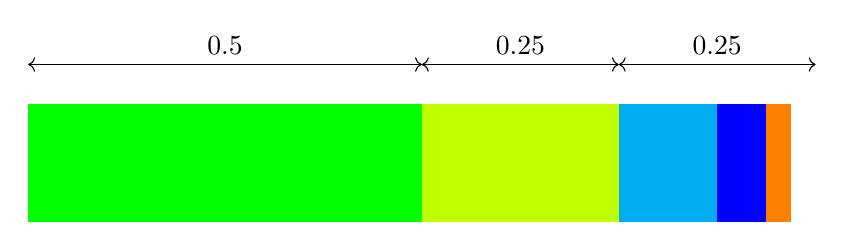
\begin{tikzpicture}
	\fill[green] (0,0) rectangle (5,1.5);
	\draw[<->](0,2) -- node[above] {$0.5$}  (5, 2);
	\onslide<2->{
		\fill[lime] (5,0) rectangle (7.5,1.5);
	\draw[<->](5,2) -- node[above] {$0.25$}  (7.5, 2);}
\onslide<3->{
	\fill[cyan] (7.5,0) rectangle (8.75,1.5);
	\fill[blue] (8.75,0) rectangle (9.375,1.5);
	\fill[orange] (9.375,0) rectangle (9.6875,1.5);
	\draw[<->](7.5,2) -- node[above] {$0.25$} (10, 2);}

	\draw(10,1.5);
	\end{tikzpicture}
	\end{center}
	
	
\end{frame}

\iffalse 

\begin{frame} 
	\frametitle{Jelly Beans}
	\only<1>{
		Box with one jelly bean:
		\vspace{3em}
		\begin{center}
			
\begin{tikzpicture}
				\fill[lime] (0,0) ellipse (0.7cm and 0.5cm);
			\end{tikzpicture}
		\end{center}
	}
	
	\only<2->{
		Box with more jelly beans:
		\vspace{5em}
		\begin{center}
			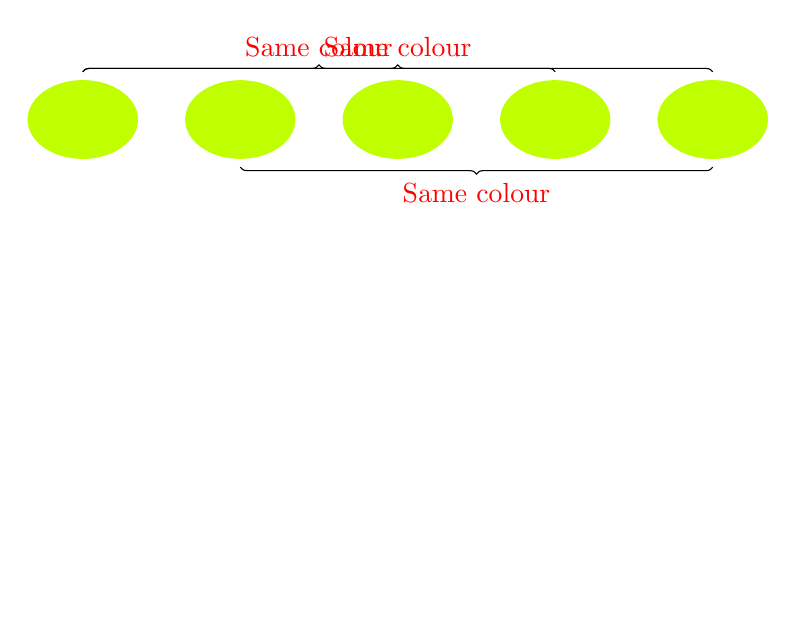
\begin{tikzpicture}
				\draw(0,-6);
				\onslide<2-3>{\draw[decoration={brace, raise={4ex}}, decorate] (0,0) -- node[above,yshift=4.5ex, red] {Same colour} (6,0);}
				
				\onslide<3>{\draw[decoration={brace, raise={4ex}}, decorate] (8,0) -- node[below,yshift=-4.5ex, red] {Same colour} (2,0);}
				
				\onslide<1-3>{\fill[lime!60] (0,0) ellipse (0.7cm and 0.5cm);}
				\fill[lime] (2,0) ellipse (0.7cm and 0.5cm);
				\fill[lime] (4,0) ellipse (0.7cm and 0.5cm);
				\fill[lime] (6,0) ellipse (0.7cm and 0.5cm);
				\onslide<1-3>{\fill[lime!60] (8,0) ellipse (0.7cm and 0.5cm);}
				\onslide<4> {
					\draw[decoration={brace, raise={4ex}}, decorate] (0,0) -- node[above,yshift=4.5ex, red] {Same colour} (8,0);
					\fill[lime] (0,0) ellipse (0.7cm and 0.5cm);
					\fill[lime] (8,0) ellipse (0.7cm and 0.5cm);
					
				}
			\end{tikzpicture}
		\end{center}
	}
\end{frame}
\fi

\section{Project Background} 
\begin{frame}
		\frametitle{Programming Languages}
		Calculating $5 + 3 * 2$. 
		\vspace{1em}
		\pause 
			\begin{center}
			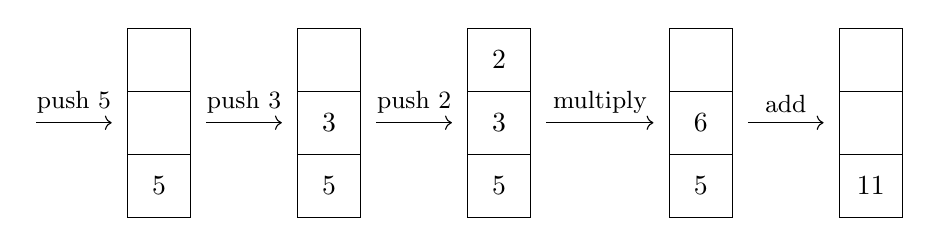
\begin{tikzpicture}[scale=0.8]
				\begin{scope}[shift = {(-1.25, 0)}] 
					\draw [-> ] (1.25, 1.5) -- node[above] {\small push 5} (2.45, 1.5); 
					
					\begin{scope}[shift={(2.7, 0)}]
						\draw (0,0) rectangle (1,1) node[pos=.5] {5};
						\draw (0,1) rectangle (1,2);
						\draw (0,2) rectangle (1,3);
						\draw [-> ] (1.25, 1.5) -- node[above] {\small push 3} (2.45, 1.5); 
					\end{scope}
					
					\begin{scope}[shift={(5.4, 0)}]
						\draw (0,0) rectangle (1,1) node[pos=.5] {5};
						\draw (0,1) rectangle (1,2) node[pos=.5] {3};
						\draw (0,2) rectangle (1,3);
						\draw [-> ] (1.25, 1.5) -- node[above] {\small push 2} (2.45, 1.5); 
					\end{scope}
					
					\begin{scope}[shift={(8.1, 0)}]
						\draw (0,0) rectangle (1,1) node[pos=.5] {5};
						\draw (0,1) rectangle (1,2) node[pos=.5] {3};
						\draw (0,2) rectangle (1,3) node[pos=.5] {2};
						\draw [-> ] (1.25, 1.5) -- node[above] {\small multiply} (2.95, 1.5); 
					\end{scope}
					
					\begin{scope}[shift={(11.3, 0)}]
						\draw (0,0) rectangle (1,1) node[pos=.5] {5};
						\draw (0,1) rectangle (1,2) node[pos=.5] {6};
						\draw (0,2) rectangle (1,3);
						\draw [-> ] (1.25, 1.5) -- node[above] {\small add} (2.45, 1.5); 
					\end{scope}
					
					\begin{scope}[shift={(14, 0)}]
						\draw (0,0) rectangle (1,1) node[pos=.5] {11};
						\draw (0,1) rectangle (1,2);
						\draw (0,2) rectangle (1,3);
					\end{scope}
				\end{scope}
				
			\end{tikzpicture}
		\end{center}
\end{frame}	

\begin{frame}[fragile]
	\frametitle{Programming Languages}
	\begin{minted}[numbersep=5pt,gobble=0,frame=lines,framesep=2mm,breaklines]{c}
static void cmd_backup(struct userrec *u, int idx, char *par)
{
	putlog(LOG_CMDS, "*", "#%s# backup", dcc[idx].nick);
	dprintf(idx, "Backing up the channel & user files...\n");
	call_hook(HOOK_BACKUP);
}
	\end{minted}
\end{frame}

\begin{frame}[fragile]
	\frametitle{Programming Languages}
	\begin{minted}[numbersep=5pt,gobble=0,frame=lines,framesep=2mm,breaklines]{Haskell}
powerset = filterM (\_ -> [True, False])
	\end{minted}
\end{frame}
		
\begin{frame} 
		\frametitle{The Obvious}
		\begin{itemize}
			\item<2-> ``Roses are red and violets are blue'' is logically equivalent to ``Violets are blue and roses are red''
			\item<3-> $2 + 3 = 5$
			\item<4-> $a + b = b + a$ 
			\item<5-> $1 \neq 2$
		\end{itemize}
		\epigraph{Some of our fellow sinners are among the most careful and competent logicians on the contemporary scene.}{Haskell B. Curry and Robert Feys}
\end{frame}

\begin{frame}
	\frametitle{Applications} 
	\begin{columns}
\begin{column}{0.5\textwidth}
		\begin{itemize} 
		\item<2-> New languages can reduce labour
		\item<3-> New languages and theorem provers can eliminate bugs
		\begin{itemize} 
			\item<4-> \$59 billion loss per year in US
			\item<5-> Death
		\end{itemize}
	\end{itemize}
\end{column}   
\begin{column}{0.5\textwidth}
	\begin{figure}
		\centering
		\includegraphics[width=0.7\textwidth]{ariane}
	\end{figure}
\end{column}
\end{columns}
\end{frame}

\section{Foundations of Mathematics} 

\begin{frame}
	\frametitle{Meta-Languages} 
	\vspace{2em}
	\begin{columns}[c]
	\begin{column}{0.30 \textwidth}
		\uncover<2-> {
		 
		 \[
		 \begin{prooftree}
		 	\hypo{A}
		 	\hypo{B}
		 	\infer2[$(\land I)$]  {A \land B}
		 \end{prooftree}
		 \]
		 
		 \[
		 \begin{prooftree}
		 	\hypo{A \land B}
		 	\infer1[$(\land E_1)$]  {A}
		 \end{prooftree}
		 \]
		 
		 \[
		 \begin{prooftree}
		 	\hypo{A \land B}
		 	\infer1[$(\land E_2)$]  {B}
		 \end{prooftree}
		 \]
		} 
	\end{column}
	\vline{}
	\begin{column}{0.50 \textwidth}
		\uncover<3->{
		\[
		\begin{prooftree} 
			\hypo{A \land B}
			\infer1[($\land E_2$)]{B}
			\hypo{A \land B}
			\infer1[($\land E_1$)]{A}
			
			\infer2[($\land I$)]{B \land A}
		\end{prooftree}
		\]
	}
	\end{column}
\end{columns}
\end{frame}
\begin{frame} 
	\frametitle{$\lambda$-Calculi}
     Proof languages are often based off the $\lambda$-calculus. 
     \only<2>{
     \begin{align*}
     	T = \underbrace{\lambda x .}_{\text{\textcolor{red}{Abstraction}}} \lambda y . x\\
     	F = \lambda x. \lambda y. y\\
     	N = \lambda b. \underbrace{b\ F\ T}_{\text{\textcolor{blue}{Application}}}
     \end{align*}
 	}
     \only<3>{
    	\begin{align*}
    		& (\lambda b. b \ F \ T) (\lambda x. \lambda y. y)\\
    		\textcolor{blue}{\to} \ & (\lambda x. \lambda y. y)\ F \ T\\ 
    		\textcolor{blue}{\to} \ & T
    	\end{align*}
    } 
   
     
\end{frame}

    \section{The Language}  
    
    \begin{frame}
    	\frametitle{Formal Language Theory} 
    	\vspace{2em}
    		\begin{columns}[c]
    		\begin{column}{0.60 \textwidth}
    			\uncover<2-> {
    		
    				
    				\begin{grammar}
    					\centering 
    					<add> $\rightarrow$ <var> "+" <add> | <mult>
    					
    					<mult> $\rightarrow$ <var> "*" <mult> | "(" <add> ")" | <var>
    					
    					<var> $\rightarrow$ "a" | "b" | "c" 
    				\end{grammar} 
    		
    			} 
    		\end{column}
    		\vline{}
    		\begin{column}{0.30 \textwidth}
    			\only<3>{
    				\centering
    				   	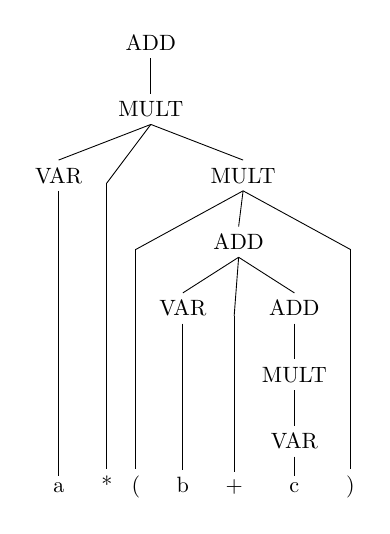
\begin{tikzpicture}[scale=0.8]
    					\tikzset{frontier/.style={distance from root=200pt}}
    					\Tree [.ADD [.MULT [.VAR a ] [* ] [.MULT [ ( ] [.ADD [.VAR b ] [+ ] [.ADD [.MULT [.VAR c ] ] ] ] [ ) ] ]  ] ]
    				\end{tikzpicture}
    			}
    			\only<4>{
    				\centering
    				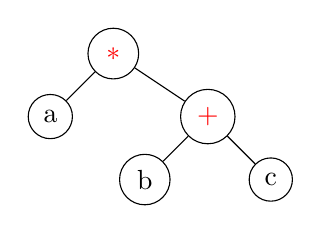
\begin{tikzpicture}[scale=0.8]
    					\node[circle,draw, label={[yshift=-0.17em,red]center:*}] (mult) at (0,0) {\phantom{*}}; 
    					\node[circle,draw] (a) at (-1,-1) {a}; 
    					\node[circle,draw, text = red] (plus) at (1.5,-1) {+}; 
    					\node[circle,draw] (b) at (0.5,-2) {b}; 
    					\node[circle,draw] (c) at (2.5,-2) {c}; 
    					\draw (mult) -- (a);
    					\draw(mult) -- (plus); 
    					\draw (plus) -- (b); 
    					\draw (plus) -- (c);
    				\end{tikzpicture}
    			}
    			
    			
    		\end{column}
    	\end{columns}
    	 \end{frame}
    	\begin{frame}
    		\frametitle{Implementation Details} 
			\begin{columns}[c]
    		\begin{column}{0.40 \textwidth}
           	\begin{itemize}
           		\item<2-> The language is parsed 
           		\item<3-> Definitions across files are resolved
           		\item<4-> Definitions are topologically sorted
           		\item<5-> Type-checking is done
           	\end{itemize}
           \end{column} 
       \begin{column}{0.60 \textwidth}
       	\centering
       		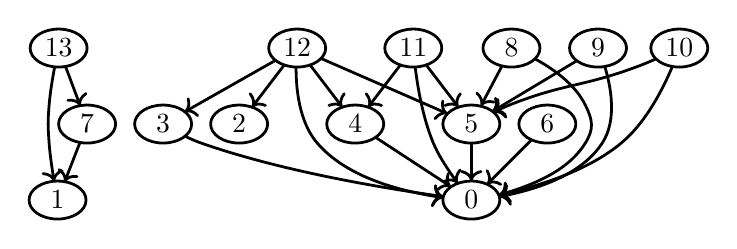
\begin{tikzpicture}[line join=bevel,scale=0.38]
	\pgfsetlinewidth{1bp}
	%%
	\pgfsetcolor{black}
	% Edge: 40 -> 39
	\draw [->] (48.222bp,72.571bp) .. controls (45.013bp,64.319bp) and (41.106bp,54.274bp)  .. (33.813bp,35.518bp);
	% Edge: 41 -> 39
	\draw [->] (24.253bp,144.09bp) .. controls (22.253bp,133.62bp) and (20.003bp,120.12bp)  .. (19.0bp,108.0bp) .. controls (17.68bp,92.055bp) and (17.824bp,87.957bp)  .. (19.0bp,72.0bp) .. controls (19.627bp,63.493bp) and (20.802bp,54.294bp)  .. (23.668bp,35.926bp);
	% Edge: 41 -> 40
	\draw [->] (34.674bp,144.2bp) .. controls (37.748bp,136.01bp) and (41.462bp,126.1bp)  .. (48.403bp,107.59bp);
	% Edge: 1 -> 0
	\draw [->] (147.93bp,78.413bp) .. controls (152.78bp,76.047bp) and (157.99bp,73.75bp)  .. (163.0bp,72.0bp) .. controls (238.67bp,45.592bp) and (331.65bp,29.934bp)  .. (392.23bp,21.348bp);
	% Edge: 2 -> 0
	\draw [->] (328.41bp,77.294bp) .. controls (345.74bp,65.951bp) and (371.33bp,49.201bp)  .. (399.41bp,30.822bp);
	% Edge: 3 -> 0
	\draw [->] (419.0bp,71.831bp) .. controls (419.0bp,64.131bp) and (419.0bp,54.974bp)  .. (419.0bp,36.413bp);
	% Edge: 4 -> 0
	\draw [->] (479.53bp,151.61bp) .. controls (496.03bp,142.64bp) and (517.18bp,127.97bp)  .. (527.0bp,108.0bp) .. controls (534.06bp,93.641bp) and (535.41bp,85.61bp)  .. (527.0bp,72.0bp) .. controls (511.4bp,46.767bp) and (480.05bp,32.93bp)  .. (445.25bp,22.929bp);
	% Edge: 4 -> 3
	\draw [->] (447.99bp,144.94bp) .. controls (443.52bp,136.45bp) and (438.0bp,126.01bp)  .. (428.2bp,107.44bp);
	% Edge: 5 -> 0
	\draw [->] (545.41bp,144.5bp) .. controls (551.32bp,125.11bp) and (557.23bp,93.717bp)  .. (543.0bp,72.0bp) .. controls (523.78bp,42.66bp) and (484.76bp,29.174bp)  .. (445.75bp,21.149bp);
	% Edge: 5 -> 3
	\draw [->] (518.91bp,149.95bp) .. controls (499.45bp,138.27bp) and (469.72bp,120.43bp)  .. (439.15bp,102.09bp);
	% Edge: 6 -> 0
	\draw [->] (609.36bp,144.37bp) .. controls (600.96bp,124.27bp) and (584.67bp,91.649bp)  .. (561.0bp,72.0bp) .. controls (530.19bp,46.422bp) and (485.97bp,32.189bp)  .. (445.17bp,22.607bp);
	% Edge: 6 -> 3
	\draw [->] (593.65bp,151.6bp) .. controls (587.65bp,148.97bp) and (581.13bp,146.25bp)  .. (575.0bp,144.0bp) .. controls (522.74bp,124.77bp) and (506.76bp,128.53bp)  .. (455.0bp,108.0bp) .. controls (453.15bp,107.27bp) and (451.26bp,106.47bp)  .. (440.04bp,101.28bp);
	% Edge: 7 -> 42
	\draw [->] (241.52bp,145.66bp) .. controls (234.49bp,136.46bp) and (225.57bp,124.78bp)  .. (211.43bp,106.27bp);
	% Edge: 7 -> 0
	\draw [->] (252.97bp,143.89bp) .. controls (252.83bp,123.95bp) and (255.67bp,92.064bp)  .. (273.0bp,72.0bp) .. controls (300.41bp,40.254bp) and (348.25bp,27.153bp)  .. (391.97bp,20.263bp);
	% Edge: 7 -> 1
	\draw [->] (233.31bp,150.27bp) .. controls (212.46bp,138.45bp) and (180.09bp,120.1bp)  .. (147.68bp,101.72bp);
	% Edge: 7 -> 2
	\draw [->] (266.48bp,145.66bp) .. controls (273.51bp,136.46bp) and (282.43bp,124.78bp)  .. (296.57bp,106.27bp);
	% Edge: 7 -> 3
	\draw [->] (276.6bp,152.14bp) .. controls (305.07bp,139.71bp) and (354.2bp,118.27bp)  .. (396.15bp,99.972bp);
	% Edge: 8 -> 0
	\draw [->] (365.79bp,143.81bp) .. controls (368.09bp,125.19bp) and (373.03bp,95.701bp)  .. (383.0bp,72.0bp) .. controls (387.32bp,61.717bp) and (393.69bp,51.312bp)  .. (405.9bp,34.085bp);
	% Edge: 8 -> 2
	\draw [->] (351.52bp,145.66bp) .. controls (344.49bp,136.46bp) and (335.57bp,124.78bp)  .. (321.43bp,106.27bp);
	% Edge: 8 -> 3
	\draw [->] (376.48bp,145.66bp) .. controls (383.51bp,136.46bp) and (392.43bp,124.78bp)  .. (406.57bp,106.27bp);
	% Edge: 9 -> 0
	\draw [->] (475.73bp,74.731bp) .. controls (465.8bp,64.803bp) and (452.68bp,51.685bp)  .. (434.25bp,33.247bp);
	% Node: 39
	\begin{scope}
		\definecolor{strokecol}{rgb}{0.0,0.0,0.0};
		\pgfsetstrokecolor{strokecol}
		\draw (27.0bp,18.0bp) ellipse (27.0bp and 18.0bp);
		\draw (27.0bp,18.0bp) node {1};
	\end{scope}
	% Node: 40
	\begin{scope}
		\definecolor{strokecol}{rgb}{0.0,0.0,0.0};
		\pgfsetstrokecolor{strokecol}
		\draw (55.0bp,90.0bp) ellipse (27.0bp and 18.0bp);
		\draw (55.0bp,90.0bp) node {7};
	\end{scope}
	% Node: 41
	\begin{scope}
		\definecolor{strokecol}{rgb}{0.0,0.0,0.0};
		\pgfsetstrokecolor{strokecol}
		\draw (28.0bp,162.0bp) ellipse (27.0bp and 18.0bp);
		\draw (28.0bp,162.0bp) node {13};
	\end{scope}
	% Node: 42
	\begin{scope}
		\definecolor{strokecol}{rgb}{0.0,0.0,0.0};
		\pgfsetstrokecolor{strokecol}
		\draw (199.0bp,90.0bp) ellipse (27.0bp and 18.0bp);
		\draw (199.0bp,90.0bp) node {2};
	\end{scope}
	% Node: 0
	\begin{scope}
		\definecolor{strokecol}{rgb}{0.0,0.0,0.0};
		\pgfsetstrokecolor{strokecol}
		\draw (419.0bp,18.0bp) ellipse (27.0bp and 18.0bp);
		\draw (419.0bp,18.0bp) node {0};
	\end{scope}
	% Node: 1
	\begin{scope}
		\definecolor{strokecol}{rgb}{0.0,0.0,0.0};
		\pgfsetstrokecolor{strokecol}
		\draw (127.0bp,90.0bp) ellipse (27.0bp and 18.0bp);
		\draw (127.0bp,90.0bp) node {3};
	\end{scope}
	% Node: 2
	\begin{scope}
		\definecolor{strokecol}{rgb}{0.0,0.0,0.0};
		\pgfsetstrokecolor{strokecol}
		\draw (309.0bp,90.0bp) ellipse (27.0bp and 18.0bp);
		\draw (309.0bp,90.0bp) node {4};
	\end{scope}
	% Node: 3
	\begin{scope}
		\definecolor{strokecol}{rgb}{0.0,0.0,0.0};
		\pgfsetstrokecolor{strokecol}
		\draw (419.0bp,90.0bp) ellipse (27.0bp and 18.0bp);
		\draw (419.0bp,90.0bp) node {5};
	\end{scope}
	% Node: 4
	\begin{scope}
		\definecolor{strokecol}{rgb}{0.0,0.0,0.0};
		\pgfsetstrokecolor{strokecol}
		\draw (457.0bp,162.0bp) ellipse (27.0bp and 18.0bp);
		\draw (457.0bp,162.0bp) node {8};
	\end{scope}
	% Node: 5
	\begin{scope}
		\definecolor{strokecol}{rgb}{0.0,0.0,0.0};
		\pgfsetstrokecolor{strokecol}
		\draw (539.0bp,162.0bp) ellipse (27.0bp and 18.0bp);
		\draw (539.0bp,162.0bp) node {9};
	\end{scope}
	% Node: 6
	\begin{scope}
		\definecolor{strokecol}{rgb}{0.0,0.0,0.0};
		\pgfsetstrokecolor{strokecol}
		\draw (616.0bp,162.0bp) ellipse (27.0bp and 18.0bp);
		\draw (616.0bp,162.0bp) node {10};
	\end{scope}
	% Node: 7
	\begin{scope}
		\definecolor{strokecol}{rgb}{0.0,0.0,0.0};
		\pgfsetstrokecolor{strokecol}
		\draw (254.0bp,162.0bp) ellipse (27.0bp and 18.0bp);
		\draw (254.0bp,162.0bp) node {12};
	\end{scope}
	% Node: 8
	\begin{scope}
		\definecolor{strokecol}{rgb}{0.0,0.0,0.0};
		\pgfsetstrokecolor{strokecol}
		\draw (364.0bp,162.0bp) ellipse (27.0bp and 18.0bp);
		\draw (364.0bp,162.0bp) node {11};
	\end{scope}
	% Node: 9
	\begin{scope}
		\definecolor{strokecol}{rgb}{0.0,0.0,0.0};
		\pgfsetstrokecolor{strokecol}
		\draw (491.0bp,90.0bp) ellipse (27.0bp and 18.0bp);
		\draw (491.0bp,90.0bp) node {6};
	\end{scope}
	%
\end{tikzpicture}
       	\end{column}
       \end{columns}
 
    	\end{frame}    	
    	\begin{frame}[fragile]
    		\frametitle{One is Not Two}
    		Logic definitions: 
    			\begin{minted}[numbersep=5pt,gobble=0,frame=lines,framesep=2mm,breaklines]{Coq}
bottom = forall a : Prop, a; 
not = fun a : Prop => forall b : a, bottom;
    		\end{minted}
    	\pause
    		Definition of natural numbers: 
    \begin{minted}[numbersep=5pt,gobble=0,frame=lines,framesep=2mm,breaklines]{Coq}
nat : Set; 
0 : nat; 
succ : forall a : nat, nat; 
1 = succ 0; 2 = succ 1; 
    \end{minted}
\end{frame}

    	\begin{frame}[fragile]
    		\frametitle{One is Not Two}
    		Axioms: 
    			\begin{minted}[numbersep=5pt,gobble=0,frame=lines,framesep=2mm,breaklines]{Coq}
equal : forall a : nat, forall b : nat, Prop; 
lower : forall a : nat, 
        forall b : nat, 
        forall p : equal (succ a) (succ b), equal a b;
0_ne_succ : forall a : nat, not (equal 0 (succ a));  
    		\end{minted}
\end{frame}

    	\begin{frame}[fragile]
    		\frametitle{One is Not Two}
    		The proof: 
    			\begin{minted}[numbersep=5pt,gobble=0,frame=lines,framesep=2mm,breaklines]{Coq}
1_ne_2 :  not (equal 1 2)
       =  fun p : equal 1 2 
       => let 0_eq_1 = lower 0 1 p 
       in 0_ne_succ 0 0_eq_1; 
    		\end{minted}
\end{frame}


    \iffalse 
      	\begin{frame}[fragile]
    	\frametitle{No Less Confusing}
    	Definition of existence: 
    \begin{minted}[numbersep=5pt,gobble=0,frame=lines,framesep=2mm,breaklines]{Coq}
exist = fun a : Set => fun gen : (forall b : a, Prop) => 
         forall c : Prop, 
         forall acc : (forall v : a, forall p : gen v, c), c; 
\end{minted}
	Definitions of inequalities:
	    \begin{minted}[numbersep=5pt,gobble=0,frame=lines,framesep=2mm,breaklines]{Coq}
gte = fun a : nat => fun b : nat => 
       exist nat (fun n : nat => eq (+ b n) a);
gt = fun a : nat => fun b : nat => gtEq a (succ b);
	    \end{minted}
    	\end{frame}
    \fi
    
\iffalse     
    \begin{frame}[fragile]
    	\frametitle{No Less Confusing}
    	\begin{minted}[numbersep=5pt,gobble=0,frame=lines,framesep=2mm,breaklines]{Coq}
gtImpGte 
  : forall a : nat, forall b : nat, implies (gt a b) (gte a b)
  = fun a : nat => fun b : nat => fun p : gt a b 
  => p (gte a b)
       ( fun n : nat  => fun p2 : eq (+ b (succ n)) a => 
         fun t : Prop => 
         fun acc : (forall v : nat, forall p3 : eq (+ b v) a, t) =>
         acc (succ n) p2
       );
    	\end{minted}
    \end{frame} 

\fi
    \begin{frame}[standout]
    	\frametitle{Tada!} 
    	\epigraph{The point of philosophy is to start with something so simple as not to seem worth stating, and to end with something so paradoxical that no one will believe it.}{Bertrand Russell}
    \end{frame}
   
\end{document}
